\documentclass{beamer}

\usepackage{beamerthemesplit}
\usetheme{Warsaw}
\setbeamertemplate{navigation symbols}{}
\setbeamercovered{transparent=25}

\title{Towards General Design Principles for Distributed Indexes}
\author[Sanket Patil]{Sanket Patil}

\institute{
\textbf{Advisor}: Dr. Srinath Srinivasa\\
Open Systems Laboratory \\ 
			International Institute of Information Technology\\
			Bangalore\\
			India		
			
			}

%\date[OT]{International Conference on Intelligent Systems - 2005\\December 3, 2005}

\begin{document}

\frame {\titlepage}

\section[Outline]{}
	\frame{\tableofcontents}

\section{Introduction}
\frame
{
	\frametitle{Introduction}
}
		
	\subsection*{Distributed Indexes}	
			\frame
				{
				\frametitle{Distributed Indexes}
				\begin{itemize}
					\item<1-> {Central to the viability of DIS}
					\item<2-> {Facilitate efficient routing of data}
					\item<3-> {Enable communication (for applications) and navigation (for users)}
					\item<4-> {Examples: distributed hash tables (DHTs), routing tables, hyperlink graphs}
				\end{itemize}				
				}
				
			\frame{
			
				%\begin{itemize}
					Design of \textit{optimal Distributed Indexes} is essential for the success of DIS
				%\end{itemize}
			}	
			

	\subsection*{Optimal Indexes: Trade-offs}
		\frame
			{
			\frametitle{Optimization: Trade-offs}
			\begin{itemize}
				\item<1-> {Minimize network diameter}
				
				\item<2-> {Minimize infrastructure cost}
				
				\item<3-> {Minimize ``book keeping'' cost}
				
				\item<4-> {Maximize load distribution}
			\end{itemize}
			}
			
			\frame
			{
			\frametitle{The Problem}
			Given $n$ nodes, find the \textbf{minimum diameter} topology under arbitrary constraints on \textbf{maximum degree}, \textbf{maximum number of edges} and \textbf{load distribution.}
			}
			
			\frame
			{
			\frametitle{Some notes}
				\begin{itemize}
			          \item<1-> {Undirected graphs}
				  \item<1-> {$n$ is a power of 2}
				\end{itemize}
			}
			
			\frame
			{	
			\frametitle{Example: Star}		
				\begin{centering}			
					\begin{figure}
						\includegraphics[height=1in]{star}
					\end{figure}
				\end{centering}	
				
				\begin{itemize}
					\item Low diameter, low infrastructure cost
					
					\item Low load distribution
				\end{itemize}	
			}
						
			\frame
			{
				Design of distributed index topology as a general optimization problem involving multiple arbitrary constraints
			}
			
			\subsection*{Evolutionary Optimization}
				\frame
				{
					\frametitle{Evolutionary Optimization}
					\begin{itemize}
						\item<1-> {Topology design as an evolutionary optimization problem}
						
						\item<2-> {Objective: Minimize diameter, subject to infrastructure cost, book keeping cost and load distribution}
						
						\item<3-> {Topology Breeding}
					\end{itemize}	
				}
							
			\subsection*{Towards General Principles}
			\frame
			{
				\frametitle{Towards General Principles}
					\begin{itemize}
						\item<1-> {Not concerned about specific applications}
						
						\item<2-> {Observing and classifying topologies}
						
						\item<3-> {\textit{Mapping} between classes of topologies to classes of real world applications }
					\end{itemize}	
			}
				
\section{Breeding Optimal Diameter Topologies}
	\frame
	{
	\frametitle{Breeding Optimal Diameter Topologies}
	}
	\subsection*{Definitions}
		\frame
			{
			\frametitle{Efficiency ($\eta$)}
				\begin{itemize}
					\item {Measure of how good the diameter $d$ is}
					
					\item {$d \in \left[n - 1, 1\right]$ and $\eta \in \left[0, 1\right]$}					
	
				\end{itemize}
				
				\[ \eta = 1 - \frac{d - 1} {n - 2}\]
			
			}
			
			\frame
			{
				\frametitle{Load Distribution ($\rho$)}
					\begin{itemize}
						\item {Measured in terms of the \textit{skew} in degree distribution}
						
						\item {$skew = \hat{p} - \bar{p} \in \left[\frac{(n - 1)(n - 2)}{n}, 0\right]$ and $\rho \in \left[0, 1\right]$}
						
						\item {$\hat{p}$ - Highest degree in the graph}
						\item {$\bar{p}$ - Average degree in the graph} 
					\end{itemize}
					
					\[ \rho = 1 - \frac{n(\hat{p} - \bar{p})}{(n - 1)(n - 2)} \]	
			}
			
			\frame
			{
				\frametitle{Maximum Permissible Degree ($p$)}
				\begin{itemize}
					\item {Upper limit on the number of edges incident on a node - $p$}
					
					\item {$p$ is a measure of the book keeping cost}
				\end{itemize}
			}
			
			\frame
			{
				\frametitle{Infrastructure Cost ($k$)}
				\begin{itemize}
					\item {Measured in terms of the number of ``extra'' edges in the graph}
					
					\item {$e_{min} = n - 1$ (tree) and $\hat{e} = \frac{n(n - 1)}{2}$ (clique)}
					
					%\item<3-> {}
				\end{itemize}
				
				\[ k = \frac{e - e_{min}} {\hat{e} - e_{min}} \]
			}
	
			\frame
			{
				\frametitle{Undirected Edges}
					\begin{itemize}
						\item<1-> {Rationale: Cost of making an edge undirected or bidirected is not significant}
						\item<2-> {Directed graphs are considered separately}
						\item<2-> {DHTs use directed edges}
						
						\item<3-> {Comparison by doubling the infrastructure cost}
					\end{itemize}
			}
	
	\subsection*{Fitness Function}
		\frame
		{
		\frametitle{Fitness}
			\begin{itemize}
			 \item<1-> {Global: minimize diameter, minimize APL, maximize load distribution (Teleological problem)}
			 \item<2-> {Local: minimize separation, minimize load (Engineering problem, MAS)}
			\end{itemize}
		}

		\frame
		{
			\frametitle{Fitness Function}
				%\begin{itemize}
				%	\item
				%\end{itemize}
				
				Defined in terms of efficiency, load distribution and infrastructure cost
				
				\[ \phi = \alpha \rho + (1 - \alpha) \eta  - k , \alpha \in \left[0, 1\right] \]
				
				 $\alpha$ is a \textit{slider} between $\eta$ and $\rho$
		}	

		\subsection*{Breeding}		
		
		\frame
		{
			\frametitle{Initial Population}
				\begin{itemize}
					\item<1-> {Large number of seed graphs (10s of $n$)}
					\item<2-> {Seed graphs are generated randomly under the $p$ and $k$ constraints}
				\end{itemize}
		}
		
		\frame
		{
			\frametitle{Mating Pool}
				\begin{itemize}
					\item<1-> {Put all the connected seed graphs in the mating pool}
					\item<2-> {All pairs cross-over}
					\item<3-> {Random mutation to realign edges so that $p$ and $k$ constraints are not breached}
				\end{itemize}
		}
				
		\frame
		{
			\frametitle{New Generation}
				\begin{itemize}
					\item<1-> {Sort all connected offsprings in non-increasing order of fitness}
					\item<2-> {$80\%$ of the new population is formed by the fittest}
					\item<3-> {$20\%$ is randomly chosen from the lesser fit}
					\item<4-> {Rationale: Effort towards reducing the chances of local minima}
				\end{itemize}
		}
		
		\subsection*{A Sample Breed}
		\frame
		{
			\frametitle{A Sample Breed}
			\begin{centering}			
					\begin{figure}
						\includegraphics[height=3in,angle=90]{trees}
					\end{figure}
				\end{centering}	

		}
		
		\subsection*{Circular Skip Lists}
		\frame
		{
			\frametitle{Circular Skip Lists}
				\begin{itemize}
					\item<1-> {When $k \ge n$, we get ``circular skip lists''}
					\item<2-> {Definition: A skip list is a topology in which each
node is given one or more edges and it uses them to connect to nodes at different distances (or ``skips'') on a logical circle}
					\item<3-> {In graph theoretic terms, the graph can be organised as a Hamiltonian circuit with several chords}
				\end{itemize}
		}
		
		\frame
		{
			\begin{itemize}
				\item<1-> {A circle is the minimal skip list}
				\item<2-> {A clique is the maximal skip list}
			\end{itemize}
		}
		
\section{Analyses}
	\frame
	{
		\frametitle{Analyses}
	}
		\frame
		{
			\frametitle{$\eta$ vs $p$ for trees where $\alpha = 0$ and $n = 8, 16, 32$}
			
			\begin{centering}			
					\begin{figure}
						\includegraphics[height=2in]{EtavsP}
					\end{figure}
			\end{centering}	
			
		}
		
		\frame
		{
			\frametitle{$\rho$ vs $p$ for trees where $\alpha = 0$ and $n = 8, 16, 32$}
			
			\begin{centering}			
					\begin{figure}
						\includegraphics[height=2in]{RhovsP}
					\end{figure}
			\end{centering}	
		}
			
		\frame
		{
			\frametitle{$\eta$ and $\rho$ vs $k$ where $\alpha = 1$, $p = 4$ and $n = 32$}
			
			\begin{centering}			
					\begin{figure}
						\includegraphics[height=2in]{KvsEtaRho}
					\end{figure}
			\end{centering}		
		}
		
		\frame
		{
			\frametitle{Insight: Hamiltonian Circuits}
			\begin{itemize}
				\item<1-> {Optimal diameter topologies that balance cost and load distribution constraints (seem to) contain at least one Hamiltonian circuit}
				\item<2-> {We see circular skip lists by rearranging the topology with one of the Hamiltonian circuits forming the outer circle}
			\end{itemize}
		}
		
		\frame
		{
		\frametitle{Optimal Skip List Topologies that Emerged}
		\begin{center}
			\begin{figure}[thb]

\begin{tabular}{|c|c|c|c|c|c|l|}
\hline
Topology & $n$ & $\alpha$ & $\eta$ & $\rho$ &  $\phi$ \\
\hline
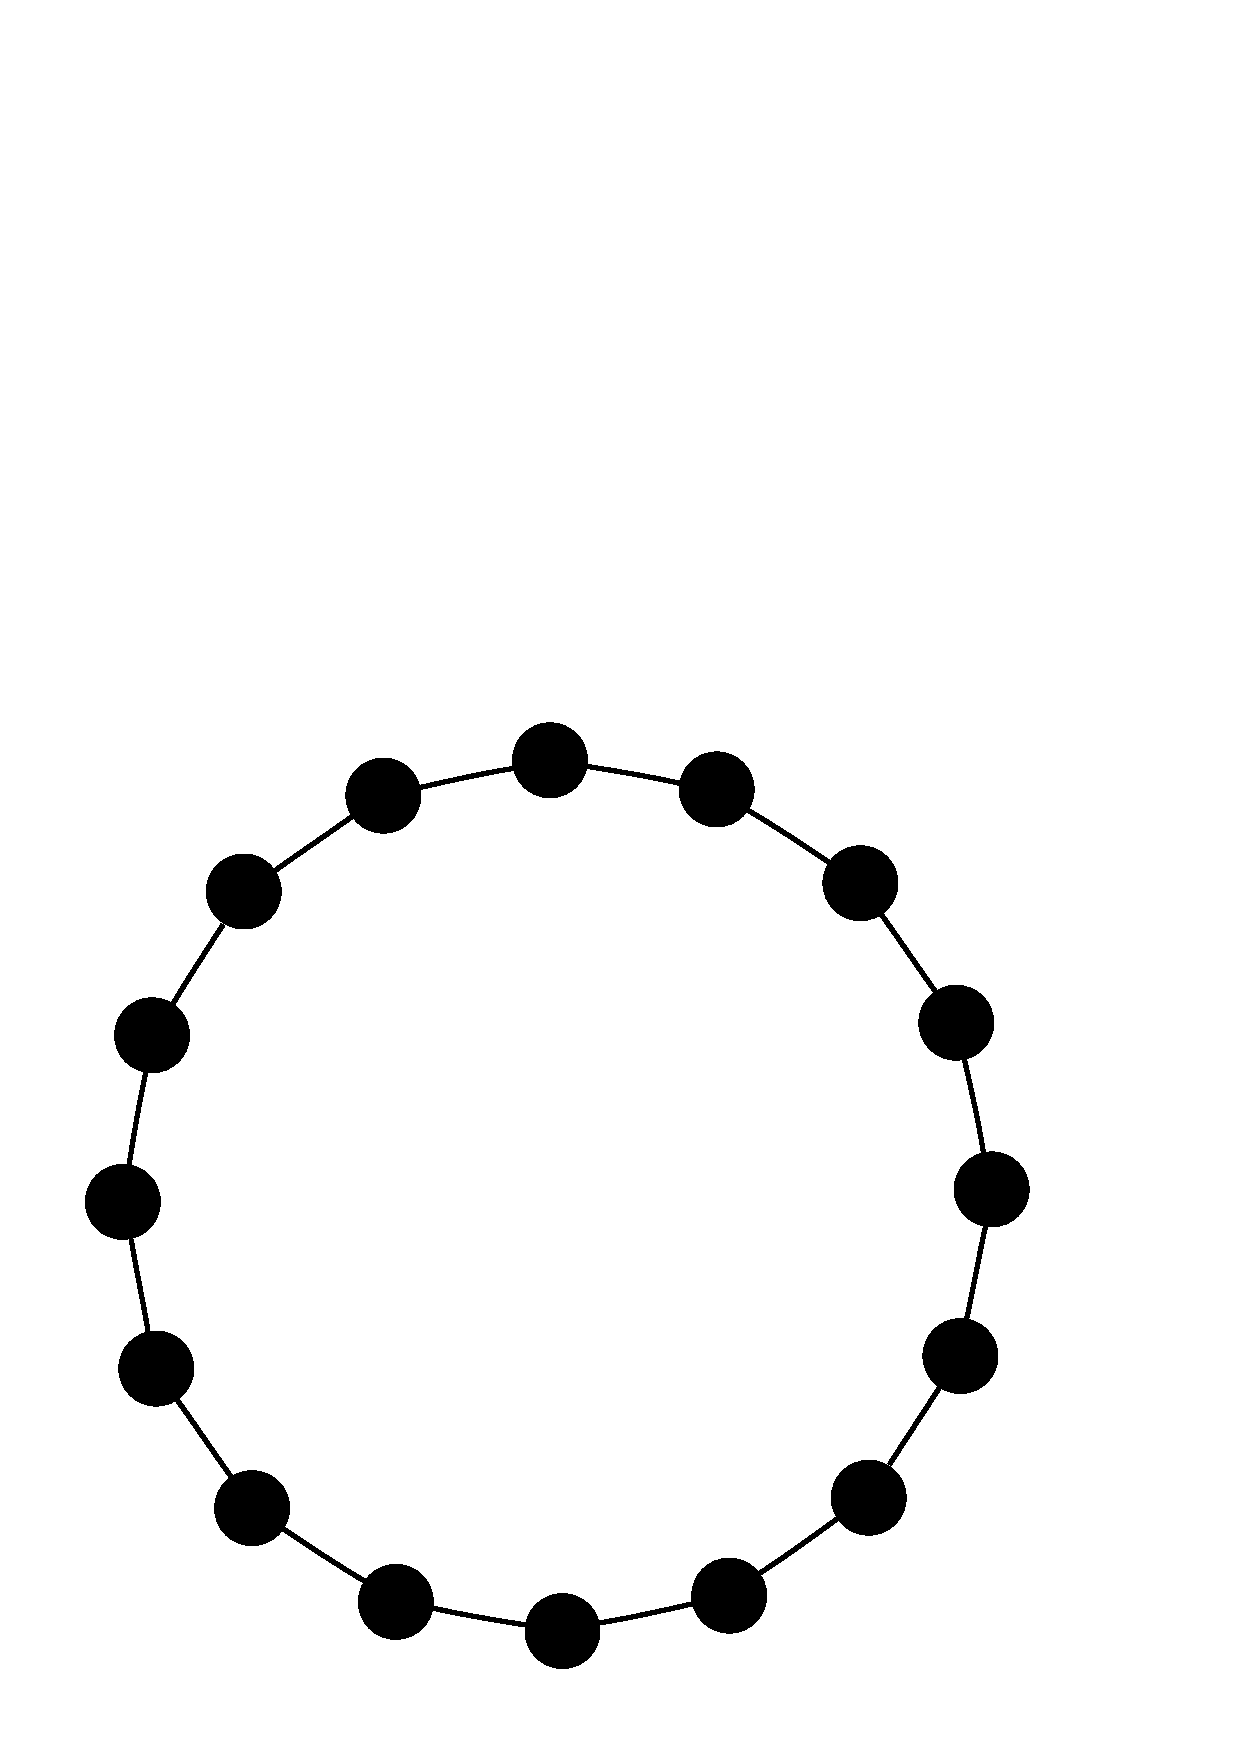
\includegraphics[width=.4in]{circle}& 16 & 1 & 0.5 & 1.0 & 1.0 \\
\hline
\includegraphics[width=.4in]{bred-topology3}& 32 & 1 & 0.9 & 1.0 & 0.95 \\
\hline
\includegraphics[width=.4in]{bred-topology2}& 64 & 1 & 0.9 & 1.0 & 0.99 \\
\hline
\includegraphics[width=.4in]{bred-topology4}& 128 & 1 & 0.97 & 1.0 & 0.98 \\
\hline
\end{tabular}
%\caption{\label{topologies} Example Optimal Topologies that are bred}
\end{figure}
\end{center}
		}
		
		\frame
		{
			\frametitle{DHTs and Hamiltonian Circuits}
			\begin{itemize}
				\item<1-> {Several existing optimal DHT topologies like the ring, butterfly and hypercube can be seen as variants of circular skip lists}
				\item<2-> {Our results corroborate DHTs}
			\end{itemize}
		}	
			\frame
			{
				Claim: an optimal distributed index topology has one or more Hamiltonian circuits
			}


\section{Polygon Embeddings with Similar Properties}
\frame
{
	\frametitle{Polygon Embeddings with Similar Properties}
}
	\subsection*{Structure and Navigability}
	\frame
	{	
		\frametitle{Structure and Navigability}
			\begin{itemize}
				\item<1-> {Difficult to predict the structure of bred topologies}
				\item<2-> {Also, difficult to find navigation patterns}
				\item<3-> {Navigability is very important for applications like distributed lookups}
				\item<4-> {Polygon Embedding: A deterministic model for building optimal diameter topologies}
			\end{itemize}		
	}
	
	\subsection*{Polygon Embedding}
	\frame
	{
		\frametitle{Single Polygon Embedding}
		\begin{centering}			
					\begin{figure}
						\includegraphics[height=2in]{polygon}
					\end{figure}
		\end{centering}
	}
	
	\frame
	{
		\frametitle{Single Polygon Embedding: Calculations}
		\begin{itemize}
			\item<1-> {It can be shown that if we embed a polygon of $l$ sides, we get a topology of diameter
	
	\[d \leq \frac{n}{l} + \frac{l}{2}\] }
		
		\item<2-> {For a given $n$ and $d$
		
			\[l \approx d - \sqrt{d^2 - 2n}\] }
		
		\end{itemize}
	}
	
	\frame
	{
		\frametitle{Single Polygon Embedding: Lower Bounds}
			\begin{itemize}
				\item<1-> {Lower bound on diameter, \[d_{lb} = \left\lceil \sqrt{2n} \right\rceil\]}
		
				\item<2-> {Size of the optimal polygon, \[l_{opt} = \left\lceil \sqrt{2n} \right\rceil\]}
				
				\item<3-> {Example: If $n = 32$, $l_{opt} = 8$ and $d_{lb} = 8$}
			\end{itemize}
	}	
	
	\subsection*{Double Polygon Embedding}
	\frame
	{
		\frametitle{Double Polygon Embedding}
			\begin{centering}			
					\begin{figure}
						\includegraphics[height=2in]{double-polygon}
					\end{figure}
			\end{centering}
	}
	
	\frame
	{
		\frametitle{Double Polygon Embedding: Lower Bounds}
		\begin{itemize}
				\item<1-> {Lower bound on diameter, \[d_{lb} = \left\lceil \sqrt{n} \right\rceil\]}
		
				\item<2-> {Size of each optimal polygon, \[l_{opt} = \left\lceil \sqrt{n} \right\rceil\]}
				
				\item<3-> {Example: a network of 256 nodes can reach a diameter of 16 by embedding two hexadecagons.}
		\end{itemize}		
	}
	
	\subsection*{Polygon Halving Embedding}
	\frame
	{
		\frametitle{Polygon Halving Embedding}
		\begin{centering}			
					\begin{figure}
						\includegraphics[height=2in]{polygon-halving}
					\end{figure}
		\end{centering}
	}
	
	\frame
	{
		\frametitle{Polygon Halving Embedding: Process}
			\begin{itemize}
				\item<1-> {Starting from an arbitrary ``root'' a polygon of size $n/2$ is embedded}
				\item<2-> {Successive embeddings are done starting from the root by halving the size}
				\item<3-> {Polygon halving embedding behaves like a tree rooted at the ``root''} 
			\end{itemize}
	}
	
	\frame
	{
		\frametitle{Polygon Halving Embedding: Diameter}
			\begin{itemize}
				\item<1-> {If the outermost embedded polygon has $l$ sides, then the diameter of the topology can be computed from the relation 

 	\[d = \frac{n}{l} + \log l\] }
 				\item<2-> {When $l = \frac{n}{2}$, as in the above example 

	\[d = \log n + 1\] }

			\end{itemize}
	}

	\subsection*{Efficiency Equivalent Polygon Embeddings}		
	
	\frame{
	\frametitle{Efficiency Equivalent Polygon Embeddings}
	\begin{center}
	\begin{figure}[thb]

\begin{tabular}{|c|c|}
\hline
Bred Topology & Polygon Embedding\\
\hline
\includegraphics[width=0.75in]{bred-topology1}& \includegraphics[width=0.75in]{similar-polygon1}\\
\hline
\includegraphics[width=0.75in]{bred-topology2}& \includegraphics[width=0.75in]{similar-polygon2}\\
\hline
\end{tabular}
%\caption{\label{equivalent-topologies} Efficiency-equivalent topologies}
\end{figure}
\end{center}
}

\frame
{
	\frametitle{Remarks}
		\begin{itemize}
			\item<1-> {In general, the evolved topologies exhibit better load distribution
than the polygon embeddings; bred topologies tend to \textit{regular graph} topologies}
		\item<2-> {Polygon embeddings are very cost effective when the desired diameter
is around the lower bounds we deduced}
	\item<3-> {They may not be cost effective for arbitrary diameters}
		\end{itemize}
}


\section{A slightly different problem...}
\frame
{
	\frametitle{A slightly different problem...}
	\begin{itemize}
	 \item<1-> {Edges per Node (epn)}
	 \item<2-> {Diameter minimization without the load distribution constraint}
	\end{itemize}
}

\feame
{
	\frametitle{The Topology Space}
	\begin{centering}			
		\begin{figure}
			\includegraphics[height=2in]{topology-space}
		\end{figure}
	\end{centering}
	
}

\section{Future Work}
\frame
{
	\frametitle{Future Work}
}

\frame
{
	\frametitle{Snapping Algorithms}
		\begin{itemize}
			\item<1-> {Families of known optimal topologies}
			\item<2-> {Given a topology, \textit{snap} on to the nearest optimal topology}
			\item<3-> {In uncertain environments, nodes can snap to the nearest optimal topologies in a distributed manner, in the face of perturbations}
		\end{itemize}
}

\frame
{
	\frametitle{PIVs}
	\begin{itemize}
	 \item<1-> {Probabilistic Incidence Vectors -- degree distribution}
	 \item<2-> {Ex: Star - [0.071, 0.071, 0.071, 0.071, 0.071, 0.071, 0.5]}
	 \item<2-> {Ex: Circle - [0.125, 0.125, 0.125, 0.125, 0.125, 0.125, 0.125, 0.125]}
	\end{itemize}
}

\frame
{
	\frametitle{Building optimal topologies}
	\begin{itemize}
         \item<1-> {PIV as a signature of an optimal topology}
         \item<2-> {PIV as an input to an arbitrary topology}
	 \item<3-> {Snap on to the nearest optimal topology}
	 \item<4-> {Distributed algorithms: Stabilization}
	\end{itemize}	
}

\section{Some Notes on Applications}
\frame
{
	\frametitle{Some Notes on Applications}
}

\frame
{
	\frametitle{Applications}
		\begin{itemize}
			\item<1-> {Distributed Hash Tables}
			\item<2-> {Mobile Collaborative Applications}
			\item<3-> {Information Architecture}
		\end{itemize}
}


\section{Conclusions}
	\frame
	{
		\frametitle{Conclusions}
			\begin{itemize}
				\item<1-> {We propose to develop general principles for designing distributed indexes}
				\item<2-> {Generic perspective to a class of problems involving topology design under different conditions}
				\item<3-> {Emergence of Hamiltonians as optimal structures}
				\item<4-> {Need to develop snapping algorithms}				
			\end{itemize}	
	}
	
\section*{Acknowledgements}
	\frame
	{
		\frametitle{Acknowledgements}
			\begin{itemize}
				\item {Infosys Technologies}				
			\end{itemize}
	}
		
\frame
{
	\frametitle{References}
}

\begin{thebibliography}{100}

\bibitem{koorde}M.F.Kaashoek and D.R.Karger. Koorde: A simple degree optimal distributed hash table. Proc. of IPTPS, 2003.
\bibitem{chord}I.Stoica, R.Morris, D.Karger, F.Kaashoek and H.Balakrishnan. Chord: A scalable Peer-To-Peer lookup service for internet applications. Proc. of ACM SIGCOMM, 2001.
\bibitem{pastry}A.Rowstron and P.Druschel. Pastry: Scalable, decentralized object location and routing for large-scale peer-to-peer systems. Proc. of the IFIP/ACM International Conference on Distributed Systems Platforms, 2001.
%\bibitem{tapestry}B. Y. Zhao, J. D. Kubiatowicz, and A. Joseph. Tapestry: An Infrastructure for Fault-Tolerant Wide-Area Location and Routing. Univ. Calfornia Berkeley Tech. Rep., Apr. 2001. 
\bibitem{loguinov}D.Loguinov, J.Casas and X.Wang. Graph-Theoretic Analysis of Structured Peer-to-Peer Systems: Routing Distances and Fault Resilience. IEEE/ACM Trans. on Networking, vol-13, no-5, pp. 1107-1120, October 2005.
%\bibitem{d2b}P.Fraigniaud and P.Gauron. An overview of the content-addressable network D2B. Proc. of ACM PODC, 2003.
%\bibitem{dist-trie}M.J.Freedman and R.Vingralek. Efficient peer-to-peer lookup based on a distributed trie. Proc. of IPTPS, 2002.
\bibitem{emergence}V.Venkatasubramanian, S.R.Katare, P.R.Patkar and F.Mu. Spontaneous
emergence of complex optimal networks through evolutionary computation.
Computers and Chemical Engineering. volume 28, pp.1789-1798, 2004. 
\bibitem{open-questions}S.Ratnasamy, S.Shenker and I.Stoica. Routing algorithms for DHTs: Some open questions. Proc. of IPTPS, 2002.
\bibitem{tsystems}V.Venkatasubramanian. A Theory of Design of Complex Teleological Systems: Unifying the Darwinian and Boltzmannian Perspectives. Complexity, 12(3), 2007
\bibitem{moore}W.G.Bridges and S.Toueg. On the impossibility of directed moore
graphs. J. Combinator. Theory, ser. B29, no. 3, pp. 339�341, 1980.
%\bibitem{plaxton}C.G.Plaxton, R.Rajaraman and A.W.Richa. Accessing nearby copies
of replicated objects in a distributed environment. Proc. of ACM SPAA, 1997.
\bibitem{pandurangan}G.Pandurangan, P.Raghavan and E.Upfal. Building low-diameter
P2P networks. Proc. of IEEE FOCS, 2001.
\bibitem{expander}C.Law and K.-Y.Siu. Distributed construction of random expander
graphs. Proc. of IEEE INFOCOM, 2003.
%\bibitem{symphony}G.S.Manku, M.Bawa and P.Raghavan. Symphony: Distributed
hashing in a small world. Proc. of USENIX Symposium on Internet Technologies and Systems, 2003.
\bibitem{xu}J.Xu, A.Kumar and X.Yu. On the fundamental tradeoffs between
routing table size and network diameter in peer-to-peer networks. IEEE
J. Sel. Areas Commun., vol. 22, no. 1, pp. 151-163, Jan. 2004.
\bibitem{ulysses}A.Kumar, S.Merugu, J.Xu and X.Yu. Ulysses: A robust, low-diameter, low-latency peer-to-peer network. In proc. of IEEE ICNP, 2003.
\bibitem{hypercup}M.Schlosser, M.Sintek, S.Decker and W.Nejdl. HyperCuP�Hypercubes, ontologies, and efficient search on P2P networks. Proc. of Workshop on Agents and P2P Computing, 2002.
\bibitem{kleinberg}J.Kleinberg. The Small World Phenomenon: An Algorithmic Perspective. Proc.of ACM STOC, 2000.
\bibitem{viceroy}D.Malkhi, M.Naor and D.Ratajczak. Viceroy: A scalable and dynamic emulation of the butterfly. Proc. of ACM PODC, 2002. 
\bibitem{pugh}W.Pugh. Skip Lists: A probabilistic alternative to
balanced trees. Communications of the ACM, 33(6), pp. 668-676, 1990.
\bibitem{gummadi}K.Gummadi, R.Gummadi, S.Gribble, S.Ratnasamy, S.Shenker and I.Stoica. The Impact of DHT Routing Geometry on Resilience and Proximity. Proc. of ACM SIGCOMM, 2003

\end{thebibliography}
		
\end{document}
